\section{Controle}
Aeronaves do tipo asa voadora normalmente apresentam coeficientes de rolagem elevados devido a presença de uma única superfície de controle sobre a asa, os elevons. Com o objetivo de garatir um RHA entre 0.07 e 0.09, valores sugeridos por (Gudmundsson) para aeronaves cargueiras, desenvolveu-se uma superfície de controle bipartida (Figura \ref{biparticao_elevons}) onde apenas a superficie interna é responsável pela rolagem. Desse modo, determinou-se que uma superfície de compreendida entre 43\% e 63\% da envergadura e 30\% da corda conseguiria suprir o requisito proporcionando um RHA de 0.08.


\begin{figure}
\caption{Bipartição dos elevons}
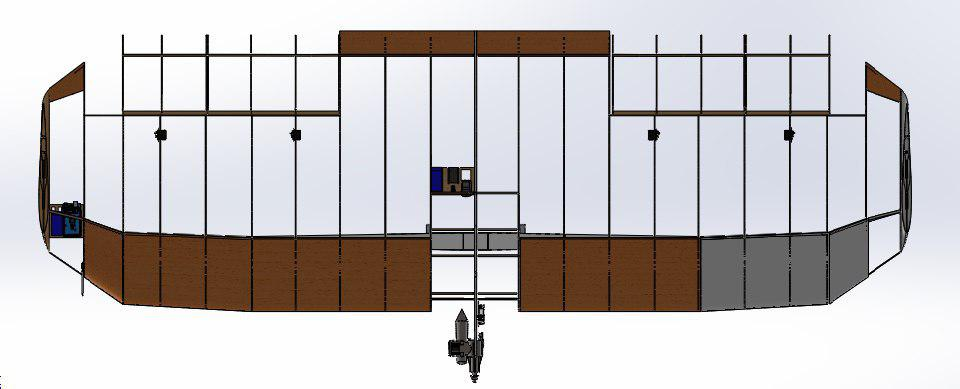
\includegraphics[scale=0.6]{RELATORIOS/Figuras/biparticao_asa.jpg}
\label{biparticao_elevons}
\end{figure}

A dimensão das superfícies para o controle de arfagem e guinada foram determinado a partir de valores históricos da equipe como 30\% da corda e 50\% da envergadura para o elevon e Leme \textit{full span} e 30\% da corda..


 
